\documentclass[a4paper]{article}
\usepackage[english]{babel}
\usepackage{setspace}
\usepackage{mathtools}
\usepackage{listings}
\usepackage[utf8]{inputenc}
\usepackage{eurosym}
\usepackage{fancyhdr}
\usepackage{tikz}
\usetikzlibrary{calc}
\usetikzlibrary{positioning}
\usetikzlibrary{arrows.meta}
\usetikzlibrary{automata}
\usetikzlibrary{fit}
\usepackage{tikzscale}
\usepackage{wrapfig}
\setcounter{secnumdepth}{-1}
\pagestyle{fancy}
\fancyhf{}
\setlength{\headheight}{24.0pt}
\lhead{Multi-Agent Systems,  Winter Semester 2018/2019, Exercise 10\\
       Submitted by: Amadeus Hovekamp, Hans Nübel, Jonathan Pieper}
\cfoot{\thepage}

\usepackage[
        colorlinks = true,    % Disable drawing boxes around links.
        linkcolor = black,    % Sets the color of links to black.
    ]{hyperref}
\definecolor{darkgreen}{rgb}{0.0, 0.5, 0.0}
\definecolor{darkred}{rgb}{0.5, 0.0, 0.0}
\newcommand{\refequation}[1]{\hyperref[#1]{(\ref{#1})}}

\begin{document}
\title{Exercise Sheet 10: Solution}
\author{}
\date{\today}

\section{Exercise 10.2}
\subsection{a)}
\begin{tikzpicture}[shorten >=1pt,node distance=5em,auto,initial text={},accepting/.style={double distance=3pt, outer sep=1.5pt+\pgflinewidth}]
\node[state] (a) {0};
\node[state] (b) [right of=a] {1};
\node[state] (c) [below of=a] {2};
\node[state] (d) [below of=b] {3};
\path[->]
    (b) edge (a)
    (c) edge (a)
    (d) edge (a)
    (d) edge (c)
;
\end{tikzpicture}
\subsection{b)}
\begin{tabular}{r||c|c|c}
Agent   & Current Value     & Agent View    & Constraint List\\\hline
0       & \color{red}1\color{black} & $\{x_1 \to 1, x_2 \to 2, x_3 \to 3\}$&$\{x_0 < x_1, x_0 \neq x_2, x_0 \neq x_3\}$\\
1       & \color{red}1\color{black} & $\emptyset$ & $\emptyset$\\
2       & \color{red}2\color{black} & $\{x_3 \to 3\}$ & $\{x_2 \neq x_3\}$\\
3       & \color{red}3\color{black} & $\emptyset$ & $\emptyset$\\
\end{tabular}\\
Agent 1 sends $(ok?, x_1 \to 1)$ to Agent 0.\\
Agent 2 sends $(ok?, x_2 \to 2)$ to Agent 0.\\
Agent 3 sends $(ok?, x_3 \to 3)$ to Agent 0.\\
Agent 3 sends $(ok?, x_3 \to 3)$ to Agent 2.\\


\begin{tabular}{r||c|c|c}
Agent   & Current Value     & Agent View    & Constraint List\\\hline
0       & \color{red}2\color{black} & $\{x_1 \to 1, x_2 \to 2, x_3 \to 3\}$&$\{x_0 < x_1, x_0 \neq x_2, x_0 \neq x_3\}$\\
1       & 1                 & $\emptyset$ & $\emptyset$\\
2       & 2                 & $\{x_3 \to 3\}$ & $\{x_2 \neq x_3\}$\\
3       & 3                 & $\emptyset$ & $\emptyset$\\
\end{tabular}\\
Agent 0 changes its number to 2 and sends $(nogood!, 0, x_2 \to 2)$ to Agent 2.\\

\begin{tabular}{r||c|c|c}
Agent   & Current Value     & Agent View    & Constraint List\\\hline
0       & 2 & $\{x_2 \to 1, x_2 \to \color{red}4\color{black}, x_3 \to 3\}$&$\{x_0 < x_1, x_0 \neq x_2, x_0 \neq x_3\}$\\
1       & 1                 & $\emptyset$ & $\emptyset$\\
2       & \color{red}4\color{black} & $\{x_3 \to 3\}$ & $\{x_2 \neq x_3, \color{red}x_2 \neq 2\color{black}\}$\\
3       & 3                 & $\emptyset$ & $\emptyset$\\
\end{tabular}\\
Agent 2 changes its number to 4 sends $(ok?, x_2 \to 4)$ to Agent 1.\\






\end{document}
